\section{Result}
\subsection{Simulation}
The simulations are based on 806 participants of ADNI study with both WGS and MRI data avaliable. Each iteration run choose a pair of testing units for genomc and image profiles. The genomic testing unit is a gene randomly picked from the genomic features list supplied by GRC38. For neuroimage profile, the testing unit is a region of 512 vertices randomly located in the cortical surface reconstructed by \FS. The genomic effect $\beta_G$ and vertex effect $\beta_G$ are then generated by randomly selecting 5\% of the variants in both types of testing unit (e.g. SNPs in a gene, and vertices in a cortical region), and assigning a value drawn from standard normal $N(0,1)$. Given the row major genomic profile $X_G$ and image profile $X_V$ of all subjects, two column vectors of continuous response $Y_G^C$ and $Y_V^C$ were calculated by adding up the element-wise products of variants and their corresponding effect across the choosen testing unit; two additional continuous responses $Y_A^C$ and $Y_I^C$ are then created by adding up the two basic ones element-wise, with or without one additional element-wise product of the two. Here, the subscripts $G$, $V$, $A$, and $I$ denote the constituents of the simulated effect originating from genomic variant only, from cortical vertices only, addition of the two, and interaction of the two, respectively; the superscript $C$ says the response is continuous. Four dichotomous responds: $Y_G^D$, $Y_V^D$, $Y_+^D$ and $Y_*^D$ were also generated by putting the four continuous ones through inverse logit and draw cases from the resulting probabilities. The generation of all 8 responses can be written as:
\begin{equation*} \label{eq:SIM}
\begin{split}
  \boldsymbol{\beta_G} &= [N_{|G|}(0,1) B_{|G|}(1, 0.05)] \\
  \boldsymbol{\beta_V} &= [N_{|G|}(0,1) B_{|V|}(1, 0.05)] \\
  \boldsymbol{Y_G^C}     &= \boldsymbol{X_G \beta_G} \\
  \boldsymbol{Y_V^C}     &= \boldsymbol{X_V \beta_V} \\
  \boldsymbol{Y_A^C}     &= \boldsymbol{Y_G^C} + \boldsymbol{Y_V^C} \\
  \boldsymbol{Y_I^C}     &= \boldsymbol{Y_G^C} + \boldsymbol{Y_V^C} + \boldsymbol{Y_G^C * Y_V^C} \\
  \boldsymbol{Y_G^D}     &= B(logit^{-1}(\boldsymbol{Y_G^C})) \\
  \boldsymbol{Y_V^D}     &= B(logit^{-1}(\boldsymbol{Y_V^C})) \\
  \boldsymbol{Y_A^D}     &= B(logit^{-1}(\boldsymbol{Y_A^C})) \\
  \boldsymbol{Y_I^D}     &= B(logit^{-1}(\boldsymbol{Y_I^C}))
\end{split}
\end{equation*}
where $N_n(\mu, \sigma^2)$ is a size $n$ sample drawn from Normal distribution of mean $\mu$ and standard variance $\sigma^2$; $B_n(1, p)$ is a size $n$ sample drawn from Bernoulli distribution of mean $p$; $|G|$ and $|V|$ denote the number of genomic variants and cortical vertices in a chosen pair of gene and cortical region, respectively. For now $|V|$ is fixed to 512.

Three factors are to be considered in the comparative study. For one, the formulation of U statistics has 3 options memtioned in the \textbf{method} section. The second factor is the construct of responses listed above. The first two factors are meant to test the performance of the U statistics when its weight kernel constituents are correctly, partially correctly, and wrongfully reflecting the effect constitution of response. Lastly, unless a purely genomic U statistic is used ($U_G$, that is), 3 constructs for the vertex bases similarity ($S_{ij}^V$) are at one's disposal: using the original vertices, the encoded vertices, or the original vertices but also the vertex-wise analysis (VWA) instead of the proposed regional aggregation. In brief, the VWA is done by first smoothing the vertex values (e.g. gray matter thickness) via a gaussian blur process, followd by the calculation of $U_V$ and $U_J$ statistics for each vertex in the testing unit. The testing unit will be declared significant if the lowest FDR (false discover rate) adjected p-value falls below the usual 0.05 threshold. All scensiable combinations of the three factors were tried out across a spectrium sample size from 100 to 800. The comparison among continuous responses is shown in Figure \ref{fig:PWR_CNT}.

\begin{figure}[h]
\centering
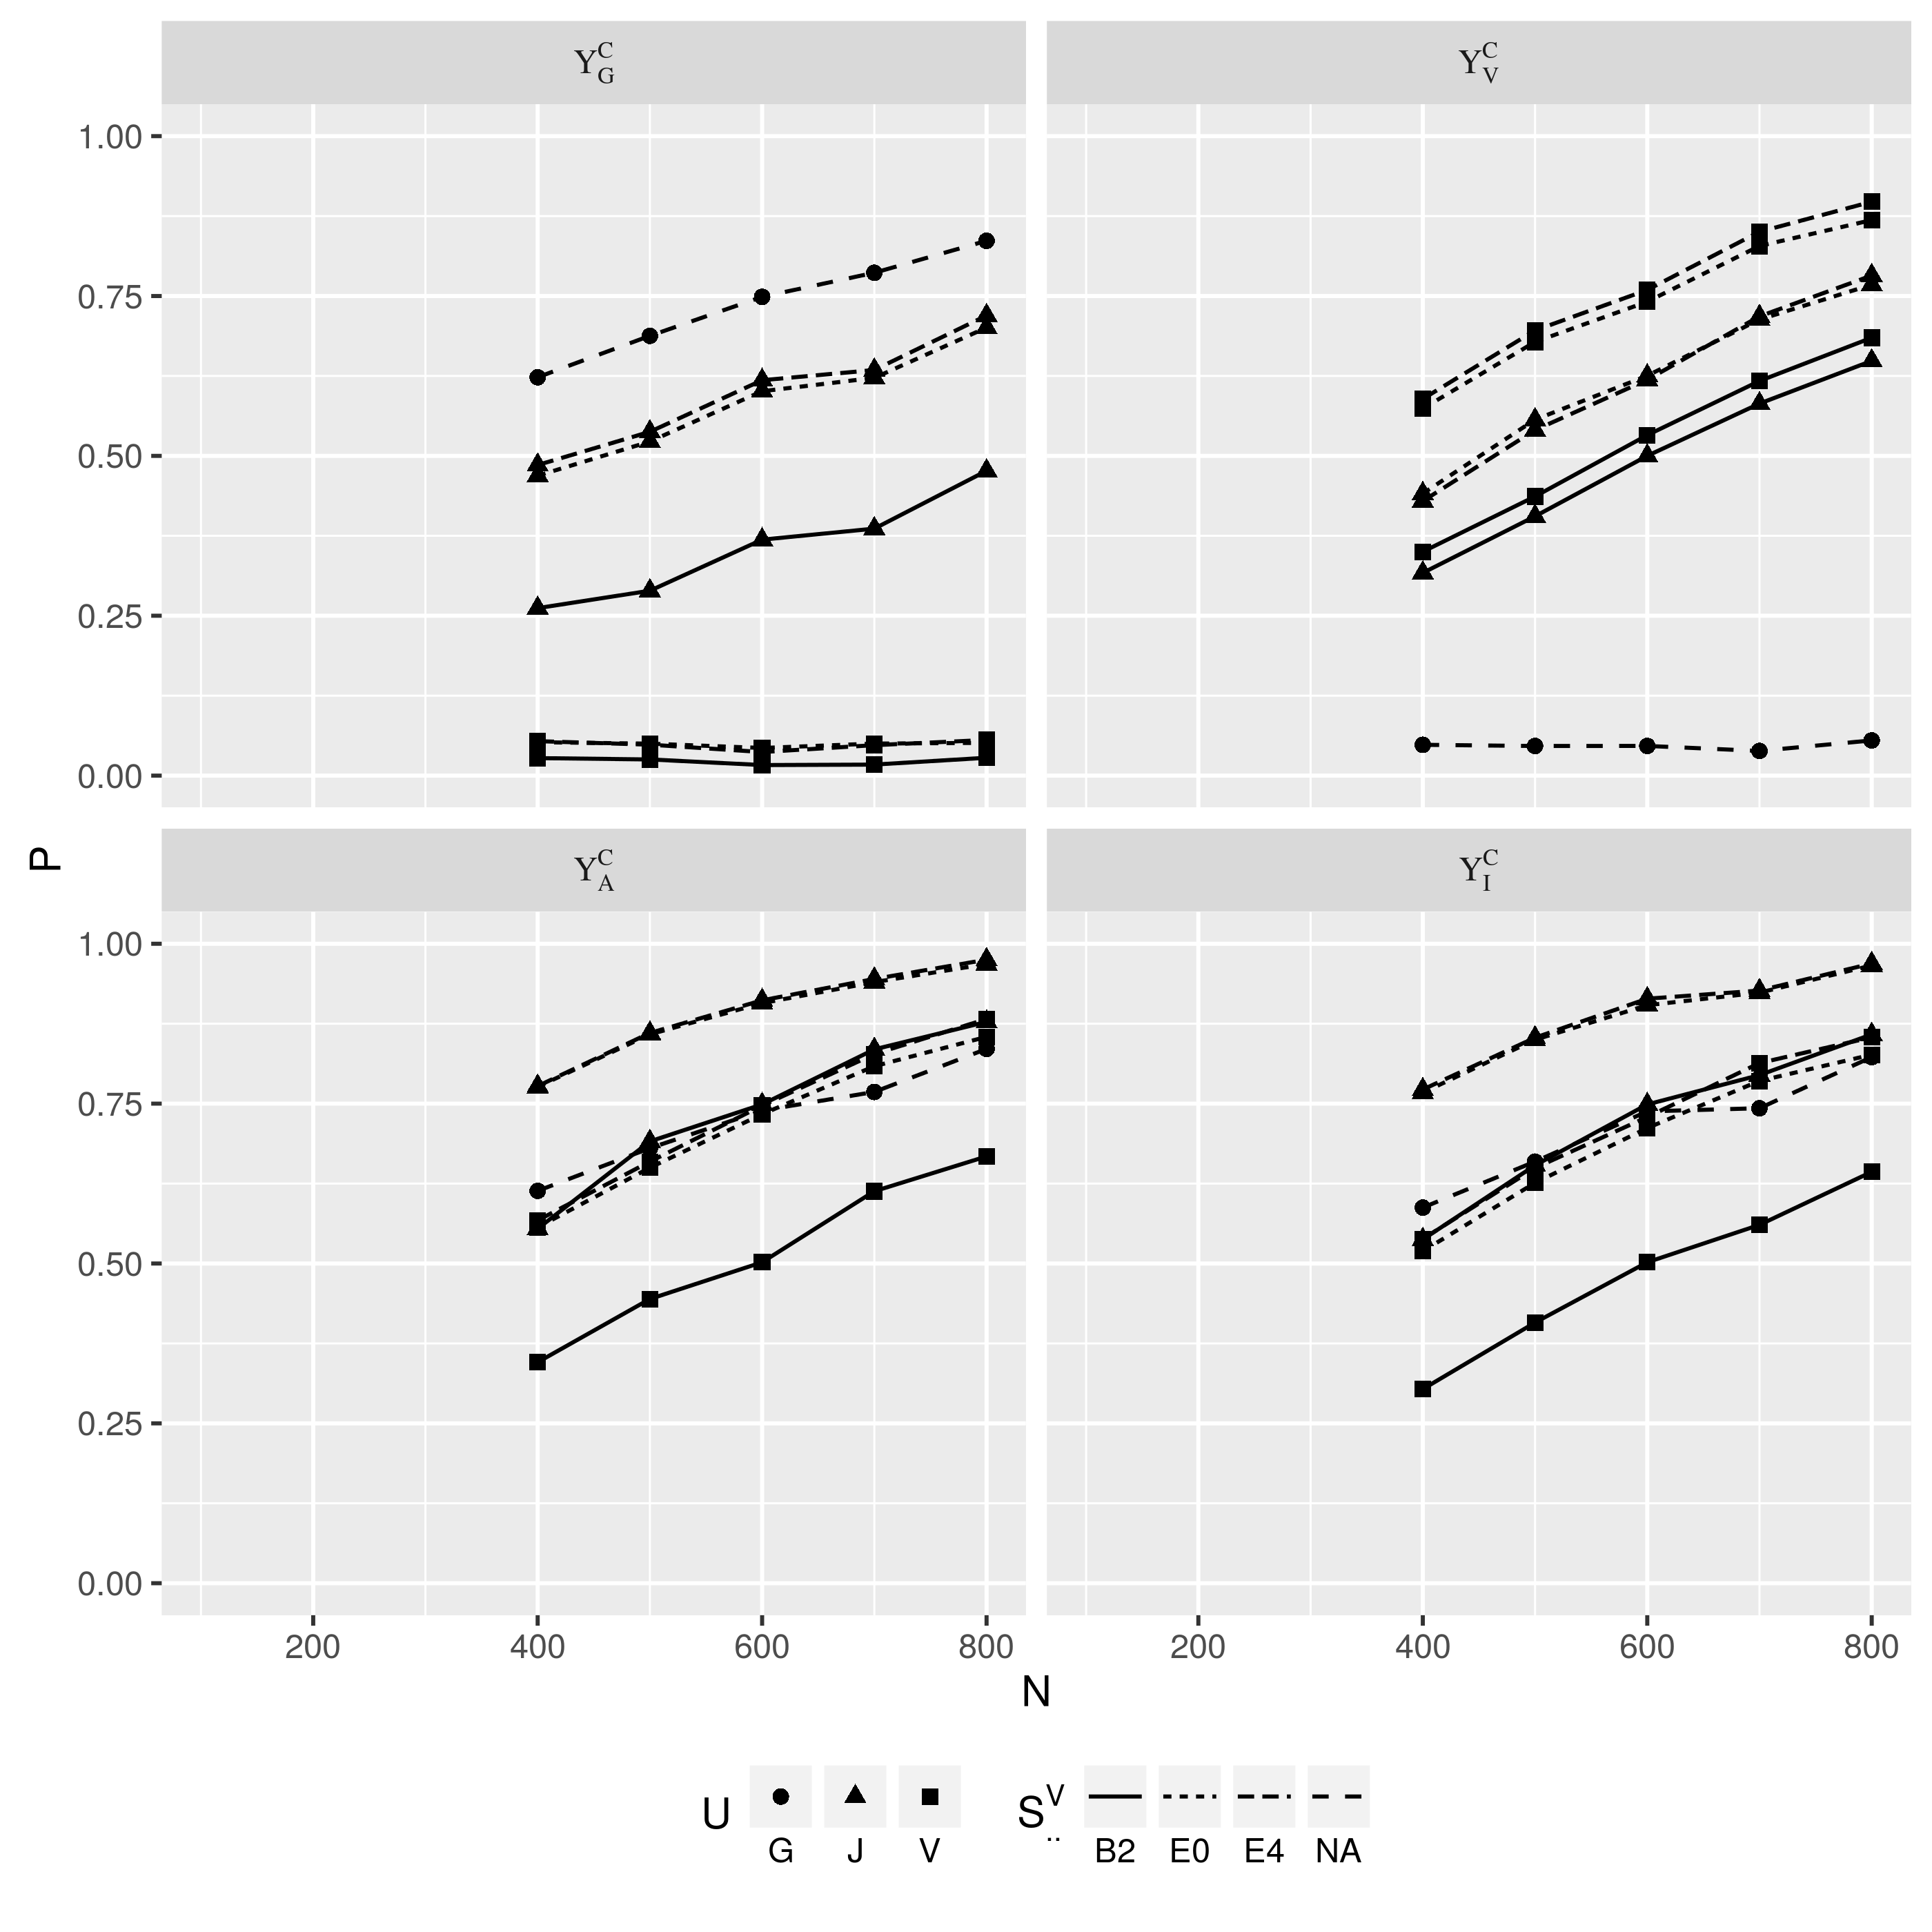
\includegraphics[width=\textwidth]{PWR_CNT}
\caption{\textbf{power performace for continuous responses}}
\label{fig:PWR_CNT}
\end{figure}

For continuous outcomes, the purely genomic profile based U statistic $U_G$ had the best performace out of the 3 when the response is chosen to be $Y_G^C$ which is also of purely genomic origin, but no power can be seen when the response is purely cortical vertex based $Y_V^C$. Conversely, the purely cortical vertex based U stistic $U_V$ displayed heighest power when the response $Y_V$, is also so constructed, and no power at all when the chosen response $Y_G^C$ was exclusively constructed from genomic variant. The joint statistics $U_J$ outperformed the two basic statistics $U_G$ and $U_V$ when the response was the additive $Y_+$ or the higher ordered $Y_I$. Between the two last responses, all 3 statistics displayed slightly higher power with the addtive $Y_I$ then with the ineractive $Y_I$. As expected, the consitution of an U statistics that better matches the underlying effect of the response should asertaine heigher power across all sample sizes, while under a scenario of complete mis-specification no statistical power should be seen. Partially mis-specified U statistics maintained a performance close to that of the perfect match, thus making the joint statistic $U_J$ an overall better choice [figure ?].
By limiting the comparesion among tests involving raw vertices, one could see that regional U statistics outperformed VWA under all circumstances except the total mis-specification where both showed no power. By only looking at regional U tests involving vertices, those employing encoded vertices would be equal or slightly underpowered at smallest sample sizes (N=100) but enjoy larger power boost alongside an constant increament in sample size. When the U statistic is correctly specified, the power is always higher if encoded vertices were used to construct $U_G$ or $U_J$. When a partial mis-specification was inccured by testing the vertex effect$Y_V$ with a joint U statistics $U_J$, where the encoded vertices outperformed the raw vertices at a higher sample size (>500), suggesting that the benefit brought by image feature abstraction could "back fire" when the statistical model is partially or fully wrong and a small sample is given. 

For dichotomous responses, the power performace shares similar patten under every circumstances, albeit universally poorer then its continuous counterpart, which is shown in Figure \ref{fig:PWR_DCT}. Another noteworthy fact is that the U statistics are indifferent to the preprocessing of the binary response thanks to the rank normal quantile standardization. The same U score are obtained regardless the U kernel being based on the deviance residual, the least squre resisual, or the binary response itself.
Nonetheless, the simulation demonstrated that the joint U statistics is an omnibus test which is more robust under most circumstances, especially when the prior knowledge of effect composition is unknown to the investigator. The feature abstration and dimension reduction is generally benificial, in that the resulting vertex code offered an accelerated power boost when sample sizes is linearly increased.

\begin{figure}[h]
\centering
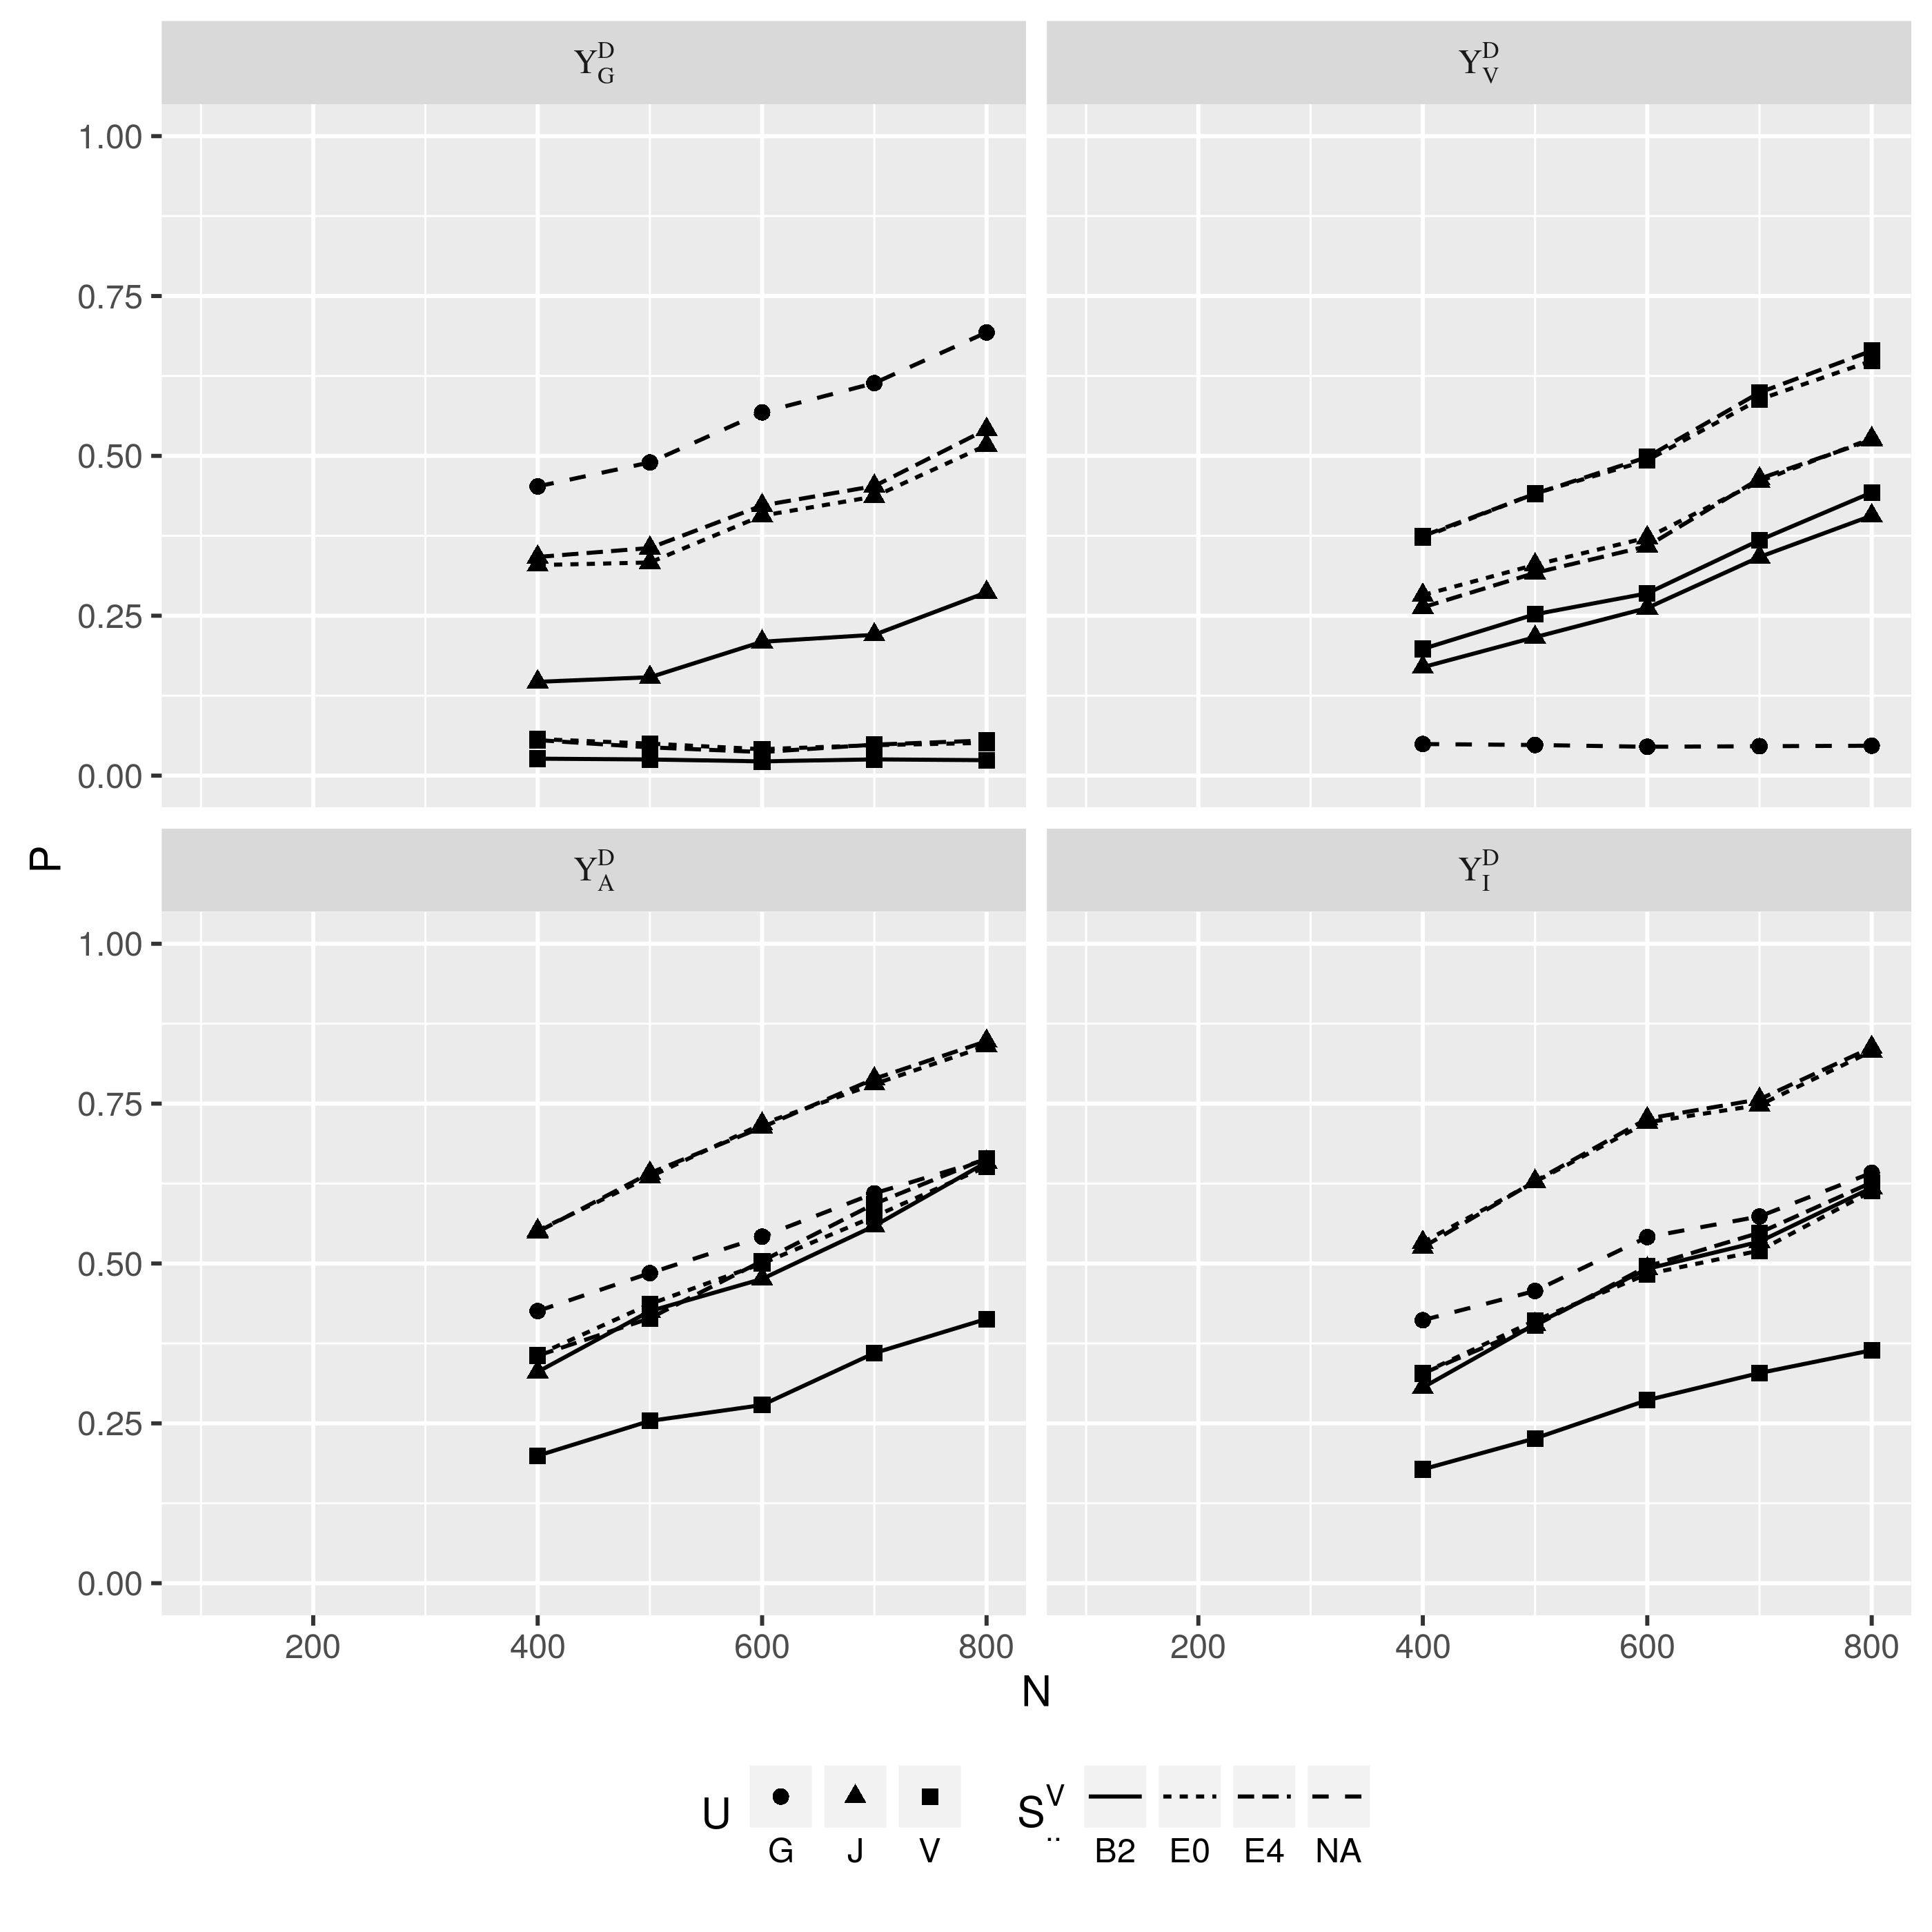
\includegraphics[width=\textwidth]{PWR_DCT}
\caption{\textbf{power performance for dichotomous responses}}
\label{fig:PWR_DCT}
\end{figure}

\subsection{real data analysis}
The baseline data of the same 806 ANDI study participants were used for the real data analysis. The genomic testing units are still genes, and thus the calculation of the corresponding similarity component $S^G_ij$ of the U statistics is the same with the simulation study. The image testing units are 68 standard anatomy regions in the cortical surface, and only the encoded vertices are used. To train the 68 encoders for these region, all 806 subjects are utilized since they all have MRI image profile. The subsequenct U statistic test only included 327 subjects comprised of 47 definite Alzheimer's disease (AD) cases and 280 healthy controls (CN). The rest 479 participants diagnosed with pre-AD or stage such as minor congitive impairment (MCI) or probable AD (PAD) were excluded from the analysis. The dichotomous outcome was first regressed on 7 known risk factors of AD, namely age, gender, race, ethnicity, years of education, marriage status, ever smoking, and APOE $\epsilon$4 allele count. The regression residuals were then taken as an continuous phenotype to construct the U kernel and weight terms. The comprehensive resuls of all 3 types of U statistics are show in Figure [?], the top 10 most significant tests are listed in table [?]. 
The results showed that the vertex based test are statistically more significance then the genome based ones, which is coherent with the fact that the neuron loss and thinning of gray matter is an proxmate indicator of the progression of Alzheimer's , while genomic profile is a remote predictor of a greater uncertainty. A noteworthy phenominium is how the joint U statistic ($U_J$) could "borrow" power from the two simpler genomic ($U_G$) and vertex ($U_V$) statistics, such that for most combinations of gene and @M regions the p-value of the joint test aligns closer to the more significant one of the two simpler U statistics, moreover, when both $U_G$ and $U_V$ are moderately significant, $U_J$ will be more so then either of them. In fact, the top 10 tests in table[?] were all from the joint U statistics $U_G$, which is the combination of the most significant WM region - left superiortemporal and the 10 most significant genes from tests $U_Vnnnn$ and $U_G$, respectively. Decection of left superiortemporal by either vertex U or joint U test is consistant with known fact that thinning of this region is a strong indicator for AD diagnosis, which is backed by ample evidences from imaging and atopsy studies [?]. The top genes so far detected couldn't remain statistically significant after multiple-testing correction and didn't contain or close to the top 20 SNPs [ref: AD SNP database] reported so far by GWAS and meta-analysis, they are likely to be due to chance. 

% latex table generated in R 3.2.3 by xtable 1.7-4 package
% Thu Feb 11 21:19:43 2016
\begin{table}[ht]
\centering
\begin{tabular}{lllll}
  \hline
  cortex & gene & $P_V$ & $P_G$ & $P_X$ \\ 
  \hline
  SFG & IGLV1-44 & 1.68e-11 & 3.51e-04 & 2.77e-13 \\ 
  SFG & NBEAP2 & 1.68e-11 & 1.19e-04 & 4.74e-13 \\ 
  SFG & RPL21P89 & 1.68e-11 & 6.36e-04 & 5.14e-13 \\ 
  SFG & LOC102724504 & 1.68e-11 & 1.41e-03 & 5.56e-13 \\ 
  SFG & CNTNAP3P8 & 1.68e-11 & 1.08e-03 & 6.17e-13 \\ 
  SFG & CDH4 & 1.68e-11 & 4.64e-03 & 6.96e-13 \\ 
  SFG & HNRNPA1P19 & 1.68e-11 & 8.88e-04 & 7.80e-13 \\ 
  SFG & FAM72C & 1.68e-11 & 9.28e-06 & 7.82e-13 \\ 
  SFG & RP11-638L3.1 & 1.68e-11 & 1.41e-01 & 9.49e-13 \\ 
  SFG & CPXM1 & 1.68e-11 & 8.78e-04 & 1.08e-12 \\ 
  SFG & LOC101929612 & 1.68e-11 & 1.44e-02 & 1.15e-12 \\ 
  SFG & LOC100996517 & 1.68e-11 & 6.77e-04 & 1.20e-12 \\ 
  SFG & IGLV5-45 & 1.68e-11 & 3.44e-04 & 1.23e-12 \\ 
  SFG & MIS18BP1 & 1.68e-11 & 4.95e-03 & 1.35e-12 \\ 
  SFG & CDR2 & 1.68e-11 & 1.82e-04 & 1.39e-12 \\ 
  SFG & RPL41P2 & 1.68e-11 & 6.04e-03 & 1.59e-12 \\ 
  SFG & LOC101927737 & 1.68e-11 & 7.20e-03 & 1.60e-12 \\ 
  SFG & IGLV1-47 & 1.68e-11 & 1.44e-02 & 1.60e-12 \\ 
  SFG & IGLV7-46 & 1.68e-11 & 9.15e-04 & 1.69e-12 \\ 
  SFG & ZDHHC15 & 1.68e-11 & 1.56e-03 & 1.73e-12 \\ 
   \hline
\end{tabular}
\caption{Top 20 combinations} 
\label{tb:tp20}
\end{table}


